\documentclass[twoside,10pt]{article}
\usepackage{shlists}
\usepackage[utf8]{inputenc}
\usepackage[spanish]{babel}
\usepackage[T1]{fontenc}


\usepackage{multicol}
\usepackage{picinpar}

\usepackage{url}
\newcommand{\surl}[1]{{\small\url{#1}}}

\newcounter{vol}
\newcounter{num}
\newcounter{anyo}
\setcounter{vol}{10}
\setcounter{num}{3}
\setcounter{anyo}{2017}
\newcommand{\mes}{Septiembre}
\usepackage{revisionNLcol}


\title{\ \\ Docencia 2.0\\ \large  Juan Julián Merelo, Fernando 
Tricas}
\author{\LARGE Paseando por las nubes}

\date{}

\AutTit{Docencia 2.0}

\begin{document}

\maketitle
\vspace*{-5ex}

\addtocounter{page}{2}
\begin{multicols}{2}

En la tensi\'on eterna entre lo local y lo remoto, el p\'endulo ha
ca\'ido ahora en lo primero y nos toca trabajar, principalmente, en la
distancia.  Es lo que nos han dicho que se llama la {\em nube}, que
m\'as all\'a de ser una especie de web, pero para hacer m\'as cosas,
es un verdadero cambio de paradigma en el desarrollo, prueba y
despliegue de sistemas inform\'aticos complejos.  Conectando una serie
de tecnolog\'ias y conceptos preexistentes, desde la concurrencia
hasta la programaci\'on funcional, hoy en d\'ia la {\em computaci\'on
en nube} es una nueva plataforma inform\'atica con un alcance similar
al que supuso el cambio de sistemas centralizados a sistemas en red o
conectados a trav\'es de Internet.

Este cambio, que ha venido sucediendo en los \'ultimos dos a\~nos, tendr\'a
que incorporarse sin m\'as remedio en la ense\~nanza universitaria de la
inform\'atica en sus diferentes grados. De hecho, los curr\'icula m\'as
recientes del IEEE y ACM, el de {\em Computer Engineering} de 2016, habla de
que uno de los resultados del aprendizaje de la asignatura {\em Sistemas
Distribuidos} (CE-CAO-11) debe ser    
\begin{quote}
  La descripci\'on de implementaciones modernas del modelo cliente
  servidor, tales como la computaci\'on basada en nube.
\end{quote}
Aunque la forma de expresarlo no acaba de capturar la esencia de la
computaci\'on en nube ni, de hecho, la computaci\'on en nube es una
implementaci\'on de ese modelo, al menos hace una menci\'on a este
paradigma y las universidades deber\'ian tomar nota. Otra asignatura,
{\em Aplicaciones en red} (CE-NWK-7) tambi\'en menciona los principios,
ventajas y retos de la computaci\'on en nube as\'i como las API de la
nube como resultados de la misma; los dos numerales que describen las
asignaturas indican, sin embargo, que son asignaturas posiblemente
optativas o en todo caso al final del grado; ninguna asignatura, de
hecho, toma la computaci\'on en nube como un concepto central o el \'unico
tema de la misma. 

Si miramos al MSIS 2017, un grado en sistemas de informaci\'on, la
computaci\'on en nube ya aparece como una de las competencias
fundamentales, la n\'umero 73; en la competencia 51, gesti\'on de
sistemas en producci\'on, tambi\'en se menciona los sistemas en nube como
una plataforma fundamental. M\'ultiples ejemplos a lo largo del
documento presentan tambi\'en diferentes servicios en la nube, o lo
mencionan en el contexto de dise\~no general de sistemas de
informaci\'on y como recursos que deben usarse para facilitar el
aprendizaje del estudiante. Este documento se extender\'a en el futuro a
dise\~nos de curr\'icula. 

Mientras tanto, en España, muchas universidades incluyen ya
expl\'icitamente computaci\'on en nube o infraestructura virtual como una
de las asignaturas, con diferente tipo de competencias; otras
asignaturas relacionadas con centros de procesos de datos tambi\'en
incluyen alg\'un tipo de temas relacionados con la virtualizaci\'on,
explicando as\'i algunas de las bases f\'isicas y tecnol\'ogicas de la
nube. Por ejemplo, la UGR tiene \emph{Infraestructura Virtual} como
asignatura en 4º de Grado, que es precisamente la que imparte uno de
los autores. 

%--------------------------
\noindent\rule{86mm}{1pt}
\vspace{1ex} 

{\small{\begin{window}[0,r,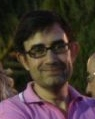
\includegraphics[width =
27mm]{JJM.jpg},] 
\noindent\emph{JJ Merelo}  es catedr\'{a}tico de Universidad
en el \'area de Arquitectura y Tecnolog\'{\i}a de Computadores. Usa,
desarrolla y promueve el software libre y todo tipo de conocimiento
abierto. 

\rule{0mm}{7ex}





\end{window}}}

\medskip

{\small{\begin{window}[0,r,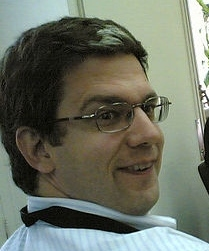
\includegraphics[width = 27
mm]{FTricas1.jpg},]
		\noindent \emph{Fernando Tricas García} es profesor
		titular de Lenguajes y Sistemas Informáticos del Departamento
		de Informática e Ingeniería de Sistemas de la Universidad de
		Zaragoza.  Empezó a estudiar la blogosfera casi cuando aún no
		existía (allá por el año 2002) y a tratar de integrarla en los
		cursos y tareas docentes un poco después.  Ha impartido
		numerosas charlas relacionadas con el tema de la Web 2.0, 
		internet y universidad,\ldots\ 
		Es actualmente Vicerrector de Tecnologías de la Información y
de la Comunicación.   
		\end{window}}}
%-------------------------------------------------



Sin embargo, pocas van m\'as all\'a explicando arquitecturas de \textsl{software},
aplicaciones nativas o una perspectiva del desarrollo de \textsl{software} centrada
en su eventual puesta en producci\'on en la nube. ?`Est\'a la ense\~nanza
universitaria preparada para ello? Es posible, pero
por lo pronto los signos de ese cambio todav\'ia no han llegado. Las
tensiones contrapuestas entre ense\~nanzas regladas que siguen un proceso
de modificaci\'on y actualizaci\'on lento y complicado y la de la libertad
de c\'atedra hace que no solo este, sino la mayor\'ia de los cambios de
paradigma en la inform\'atica tarden a\~nos, a veces muchos, en trasladarse
a los curr\'icula
universitarios. 
Tampoco la industria local favorece siempre la introducción de algunas
nuevas tecnologías y paradigmas (o al menos, de nuevas tecnologías y
paradigmas que no estén usando directamente). Eso crea, tambi\'en, una
impedancia entre los grados y
la industria que sufre ciclos, pero que aumenta de forma excesiva en
caso de cambios de paradigma como el que nos encontramos ahora
mismo. Y como la impedancia puede ir en las dos direcciones, con la
universidad impartiendo contenidos y conceptos que muchas empresas
todavía tienen que comenzar a incluir en sus procesos y negocios, es
esencial que se proporcionen medios al estudiante para disminuir esa
impedancia. 

Porque la universidad siempre ha ido m\'as all\'a de una mera
transmisi\'on de conocimientos contenidos en las enseñanzas regladas. Comunidades y clubes de
usuarios suplen, muchas veces con creces, estas ense\~nanzas,
tecnolog\'ias y conceptos que todav\'ia no han pasado por agencias de
validaci\'on y convertido en gu\'ias de estudio. Pero tanto la
universidad, como los centros y  departamentos, tienen que
potenciar y ayudar a este tipo de iniciativas, que van desde oficinas
de \textsl{software} libre hasta clubes de usuarios como el Google Developer
Club o Amazon Web Services Club por hablar de empresas bien conocidas; o
tambi\'en Databeers o los clubes .Net, 
d\'andoles alg\'un tipo de cobertura oficial tal como espacio
para reuniones o integración de talleres en un programa ``oficial'' de
seminarios. 
El objetivo será, si es posible, eventualmente y cuando tenga sentido, integrarlos de
alguna forma en el curr\'iculum m\'as formal. Pero mientras ocurra tal
cosa, el alumnado obtendr\'a
beneficios en su
futura carrera profesional y el profesorado tambi\'en, a trav\'es de la
formaci\'on continua, en la suya propia. 
Sin olvidar el factor de integraci\'on con el tejido productivo (o
proto-productivo) y los usos y costumbres. Y el aviso para alumnado y
recordatorio para profesorado de que lo \'unico
permanente es el cambio y el reciclaje, a trav\'es de diversos mecanismos,
a veces formales, y otras no tanto.


\medskip

\noindent\emph{Todas las columnas de la serie Docencia 2.0
pueden descargarse en formato LaTeX desde
\surl{https://github.com/ReVision-Docencia-20/Columnas}}

\noindent\rule{90mm}{1pt}

{\small \noindent
\includegraphics[height = 4ex]{../CC.jpg} 2017 JJ.
Merelo, F. Tricas. Este artículo es de acceso libre distribuido bajo
los términos
de la Licencia Creative Commons de Atribución, que permite copiar,
distribuir y comunicar públicamente la obra en cualquier medio, sólido
o electrónico, siempre que se acrediten a los autores y fuentes
originales}

\end{multicols}
\end{document}
